% =====================================================================
%  Chapter 11 — The State of Play, Part II
% =====================================================================

\chapter{The Two-Thirds Theorem}
\label{ch:twothirds}

Three months before the claim under examination, the same author published a
result that is the single most informative piece of context available. This
chapter is about it, because what it establishes about the method is far more
conclusive than anything that can be said about the November claim in
isolation.

\section{What was published}\begin{quote}
\textbf{Reference.} Levent Alpöge and Ralph Furman\idx{Furman, Ralph}, \emph{More than two
thirds of the zeta zeros are simple and on the critical line}, arXiv:2608.13637\idx{arXiv:2608.13637}
(13 August 2026), preprint, 33 pp.\ with appendices. The accompanying Lean
formalisation is public at \code{github.com/anthropics/formal-math} (formerly
\code{anthropics/zeta-23-lean}), submitted to the Palomar registry and
Comparator-validated according to the project's own README.
\end{quote}

The statement is a proportion theorem: more than two thirds of the zeros of
the Riemann zeta function are both \emph{simple} and \emph{on} the critical
line. It is not a proof of RH, and the paper says so --- the hypothesis remains
unproven.

\section{Why this is the crucial comparison}Three reasons, in increasing order of importance.

\begin{enumerate}
\item \textbf{It is the same method.} The argument of August 2026 and the
argument of November 2026 come from the same programme, with the same
machinery: theta lifts, the Weil--Weil positivity statement, Rallis seesaw,
Iwasawa towers. The remark's own timeline starts on 6 October 2026 --- a
\emph{month} after the two-thirds paper was posted --- and the early entries
(``Stepanov determinant'', ``$W(1S) \ge 0$ via a determinant'',
``Bost slope inequality'') are recognisably the same ideas.

\item \textbf{It is the same author, with the same collaborator.} The claim
under examination is by Levent Alpöge; the two-thirds paper is by Levent
Alpöge and Ralph Furman, and the remark's acknowledgement list includes
``especially David Dohan, Ben Michel, \textbf{Ralph Furman}, Eric Price, and
Cora Vinther''. The collaboration is continuous.

\item \textbf{It is a different answer to the same question, from the same
method.} In August, the method produced a proportion theorem. In November, the
remark's item 14 records that the method ``would stop at 2/3 a priori''. The
number 2/3 in item 14 is almost certainly the same 2/3.
\end{enumerate}

\begin{deeper}{What the comparison actually proves}
This is the part that is easy to state and easy to get wrong.

\begin{quote}
\textbf{What it proves.} The method is real. It produces rigorous,
independently reproducible, formally verified results. It was applied to the
Riemann zeta function and it yielded a statement about two thirds of the
zeros. It does not produce nonsense, and no one who had looked at the August
paper could reasonably suspect that of the November one.

\textbf{What it does not prove.} That the method can be pushed to 100 per
cent. In fact, the August paper is evidence that the method has a natural
ceiling, because it stopped there and was published as such.

\textbf{The gap.} Between ``the method works and stops at two thirds'' and
``the method works and does not stop'' there is a specific missing ingredient.
The remark's timeline suggests what it is: item 14's list of ``attempt to get
a main term and transfer constant to a function field or kill via twisting,
need for `division'''.
\end{quote}
\end{deeper}

\section{Independent reproduction}The two-thirds result was reproduced independently by a third party. Yousouf
Lamzouri\idx{Lamzouri, Yousouf}'s arXiv:2609.02882 explicitly credits ``an internal research version
of Claude developed by Anthropic'' and names ``two mathematicians at
Anthropic, Levent Alpöge and Ralph Furman'', and reproduces the same constants
by a different route.

This matters more than a mere corroboration of a number would. It means:

\begin{itemize}
\item The constants are not an artefact of one implementation.
\item The method is accessible to a specialist outside the originating group,
which is the property that distinguishes mathematics from private technique.
\item Somebody with the relevant expertise has already read the machinery, and
has reported agreement.
\end{itemize}

What it does \emph{not} mean is that the November claim has been checked. It
is a check of the August result.

\section{The record}The proportion of zeros on the critical line is a benchmark with a long
history, and the two-thirds result reset it. The figures below are the
verified records as of late 2026, and the distinctions between them matter
more than they usually do.

\begin{figure}[!htbp]
\centering
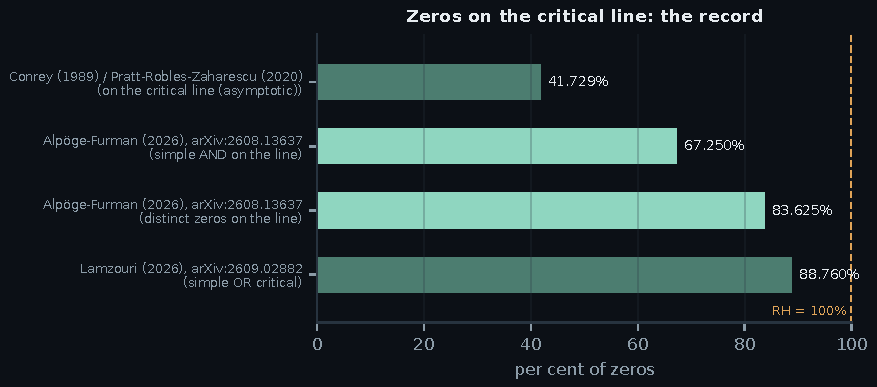
\includegraphics[width=\textwidth]{../figures/fig_records.pdf}
\caption{The verified records on the proportion of zeros on the critical
line. Note that the categories are not interchangeable: \emph{on the line},
\emph{simple and on the line}, \emph{distinct}, and \emph{simple or critical}
are four different claims, and a result in one of them is not a result in
another.}
\label{fig:records}
\end{figure}

\begin{table}[H]
\centering
\caption{Records on the proportion of zeros on the critical line.}
\label{tab:records}
\begin{tabular}{@{}p{0.30\textwidth}r p{0.40\textwidth}@{}}
\toprule
\textbf{Source} & \textbf{Proportion} & \textbf{Category} \\
\midrule
Conrey\idx{Conrey, John} (1989); Pratt--Robles--Zaharescu\idx{Pratt--Robles--Zaharescu} (2020) & 41.7293\% &
asymptotic proportion on the critical line \\
Pratt--Robles--Zaharescu (2020) & 40.7511\% &
simple \emph{and} on the critical line \\
Alpöge--Furman (2026), arXiv:2608.13637 & 67.25\% &
simple \emph{and} on the critical line \\
Alpöge--Furman (2026), arXiv:2608.13637 & 83.625\% &
distinct zeros on the critical line \\
Lamzouri (2026), arXiv:2609.02882 & 88.76\% &
simple \emph{or} critical \\
\midrule
\textbf{Riemann hypothesis} & \textbf{100\%} & all zeros, on the line \\
\bottomrule
\end{tabular}
\end{table}

The last row is not a record; it is the target. The gap between 88.76 per cent
and 100 per cent is what remains.

\section{What the two-thirds theorem tells us about the November claim}\begin{quote}
\textbf{The favourable reading.} The method works. It is rigorous. It has
been independently reproduced. It was applied by the same author with the same
machinery three months before. A method that produced a verified two-thirds
theorem is not a method that is likely to produce a wrong theorem; it is a
method that produced a right answer to a question slightly weaker than the one
now being claimed.

\textbf{The unfavourable reading.} The method stopped at two thirds, and
stopped there for a reason that the author himself computed: each theta lift
costs a third of the multiplicity it buys. A method with a per-step cost of
one third does not naturally scale to 100 per cent; it reaches two thirds and
then requires something qualitatively new.

\textbf{Which reading is right.} It depends entirely on whether the Lean
development contains that ``something qualitatively new''. That is the
question, and it is not answerable from the remark, because the remark does not
describe it.
\end{quote}

There is also a third consideration, and it cuts in favour of the favourable
reading: the two-thirds theorem was \emph{not} the plan. If the method were
known to be capable of only two thirds, a mathematician would not spend a
further three months on it and then announce a proof of the full hypothesis.
The most economical explanation of the sequence is that the extra work
produced something, and that the remark's timeline --- a ``slop'' summary,
written for a general reader, by an author who says he does not fully
understand the parts he did not do himself --- simply does not describe it.

\section{A note on what the two-thirds theorem is not}It is worth being explicit, because the press coverage of the November claim
frequently ran the two results together.

The two-thirds theorem is \emph{not} a proof of RH, a partial proof of RH, or
a proof of RH for a special case. It is a statement that a large fraction of
the zeros lie on the critical line. RH is a statement that \emph{all} of them
do. The difference between 67 per cent and 100 per cent is not a difference
of degree; it is the difference between a theorem and the conjecture.

It is also not a numerical result. It is an asymptotic statement about the
proportion of zeros as $T \to \infty$, proved analytically and formally
verified.

\begin{keytakeaways}

\item The two-thirds theorem --- arXiv:2608.13637, Alpöge and Furman, August
2026 --- is the same method, the same author, and the same programme as the
claim under examination, three months earlier.
\item It was independently reproduced by a third party, Lamzouri,
arXiv:2609.02882. It is a rigorous result, and it is the strongest positive
evidence about the method's quality.
\item It is a \emph{proportion} theorem: 67.25 per cent of zeros are simple
and on the line. It is not a proof of RH.
\item The remark's item 14 records that the method ``would stop at 2/3
a priori''. The most economical explanation of the 15-to-16 November sequence
is that the extra work produced something the remark does not describe.
\end{keytakeaways}
